
\subsection{뽀로로}

\blindtext[1]


\includegraphics[scale=0.3]{pororo}

\subsection{군침이 싹도노}

\blindtext[1]

\begin{SCfigure}[0.5][h]
	\caption{뽀로로의 친구 루피의 군침이 싹도노 명작}
	
\includegraphics[width=0.3\textwidth]{gunchim}
\end{SCfigure}

\subsection{뽀로로 텍스트 크기}

\blindtext[1]

\begin{wrapfigure}{r}{0.1\textwidth} 
	
\includegraphics[width=0.1\textwidth]{pororo}
\end{wrapfigure}

\subsection{뽀로로 사랑 ggplot}

\begin{figure}[t]
	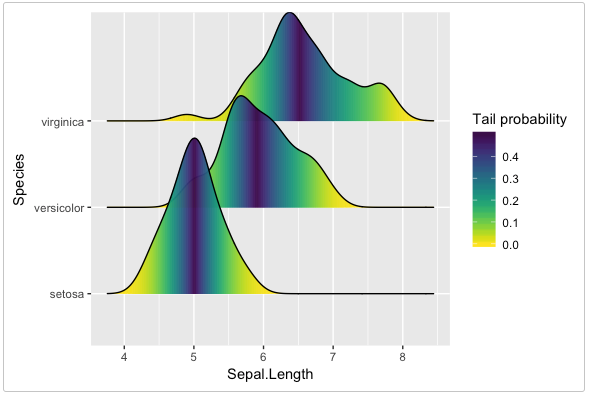
\includegraphics[width=8cm]{ggplot}
	\centering
	\caption{ggplot 시각화 }
	\label{fig:ggplot}
\end{figure}

뽀로로가 사랑한 그림 \ref{fig:ggplot} 그래프를 알아보자.

\subsection{뽀로로 크기}

\blindtext

\begin{wrapfigure}{r}{0.25\textwidth} 
	\centering
	
\includegraphics[width=0.25\textwidth]{pororo}
\end{wrapfigure}

